\sloppy

\section{Introduction}

As discussed in Chapter \ref{chapter:Introduction}, dust is composed of metals that are produced from stellar nucleosynthesis, and then expelled into the ISM via supernovae and stellar winds. While some fraction of these metals mix with the gas phase in the ISM, around $30 - 50\%$ of the metals condense into dust grains (\citealt{Draine_2007b}). If this fraction of metals that get locked up in dust grains is somewhat consistent over time, then dust may be considered a useful tracer of gas metallicity in a galaxy. For this reason, the total mass of dust in the ISM can be used to study the evolutionary stage of the galaxy (e.g. \citealt{Cortese_2012, deVis_2017a, deVis_2017b}). Moreover, dust is not just the product of previous star formation, but also, as the site of molecule formation like $H_2$, it has a significant influence on the formation of molecular clouds for future star formation. Understanding the dust content of galaxies over cosmic time is therefore important in providing insight into the evolution of galaxies and their ISM. In this Chapter, we estimate the dust masses of the galaxies in the South Galactic Pole field and derive the far-IR selected dust mass function (DMF), the space density of galaxies as a function of dust mass, in redshift slices of width $0.2$ out to $z = 1$.

\section{Local and High Redshift DMFs in the Literature}

The first direct measurements of the far-IR/sub-mm derived DMF were with SCUBA using the SCUBA Local Universe Galaxy Survey \mbox{(SLUGS: \citealt{Dunne_2000, Dunne_2001, Vlahakis_2005})}, a survey of local \textit{IRAS}-selected galaxies. However, these studies were limited by small number statistics and were typically limited to very small redshifts. A high redshift ($z = 2.5$) DMF for comparison was presented in \citealt{Dunne_2003}, suggesting that galaxies with the highest dust masses have an order of magnitude more dust than locally (assuming pure dust mass evolution and no evolution in the number density of the most massive galaxies). Improvements were made with the introduction of BLAST, which allowed for the derivation of the DMF from a sample of galaxies selected at wavelengths spanning the peak of the far-IR spectrum (the same wavelengths as the \textit{Herschel}-SPIRE instrument). \citealt{Eales_2009} used BLAST data to arrive at similar conclusions, that there is strong evolution in both the $250\,\mu$m luminosity function (LF) and in the DMF out to $z = 1$. The concurrence of the two suggesting that the evolution in the far-IR/sub-mm luminosity of these galaxies is directly related to the increase in the size of their dust reservoirs. However, this study was also limited by small number statistics ($\sim 100$ sources).

The first study to measure the evolution in the DMF using the large area of H-ATLAS was \citealt{Dunne_2011}, using a $250\,\mu$m selected sample of $1,867$ sources from the Science Demonstration Phase (SDP). This represented a sample an order of magnitude larger than previous studies, allowing for a significant direct measurement of the space-density of galaxies as a function of dust mass, out to a redshift of $0.5$. As we explored in the previous Chapter, the upper redshift limit of this study was set by the limiting magnitude of the optical surveys in the \textit{Herschel} fields. The main finding from this study was that the integrated dust density of the Universe, that is the total dust mass in a given cosmological volume, evolves with redshift according to $\rho_{\textrm{dust}} \propto (1+z)^{4.5}$ between $0 < z < 0.5$. The local density was estimated to be $\rho_{\textrm{dust}, (z=0)} = 9.8\times10^4$\,$M_\odot$Mpc$^{-3}$. This work was further developed in \citealt{Beeston_2018} where the authors derived the local ($z < 0.1$) DMF from $\sim 16,000$ galaxies, the largest H-ATLAS sample at the time of the study, using the aforementioned crossmatching between the H-ATLAS and the GAMA spectroscopic survey detailed in \citealt{Bourne_2016}. The sample size of \citealt{Beeston_2018} permitted significant numbers of galaxies with dust masses as low as $\sim 10^4\,M_\odot$ and therefore extended the observed mass range by at least an order of magnitude compared to previous measurements. This gave better constraints on the low mass end of the DMF which, despite accounting for a negligible amount of the dust budget compared to the most massive galaxies, contribute substantially in number. This low mass regime is constrained by sources that tend to be nearby and faint, and suffer from low numbers in flux-limited surveys such as H-ATLAS, thus this study provides important measurements in an otherwise uncertain region of the DMF. The large sample size of the \citealt{Beeston_2018} study means that the measurement of the low mass end of the DMF from this work is currently our best estimate. Despite differences in the measured number density of low mass galaxies, \citealt{Dunne_2011} and \citealt{Beeston_2018} both have local dust mass densities (DMD) in good agreement. More recently, \citealt{Driver_2018} produced an extended DMF and measured the DMD out to $z = 5$. This study was based on an optically-selected sample of approximately $570,000$ galaxies from GAMA, G10-COSMOS (\citealt{Davies_2015}; \citealt{Andrews_2017}) and 3D-HST (\citealt{Brammer_2012, Momcheva_2016}). Unlike \citealt{Dunne_2011}, this study found no evidence for a strong evolution in the dust content of galaxies in the past $5\,$Gyr, instead observing a flat DMD since $z = 0.5$. However, an apparent evolution is observed in the dust luminosity which would suggest that a strong evolution in dust temperature is required in order to maintain a flat DMD. Other notable works that measure the evolution of the DMF to high redshifts include \citealt{Pozzi_2020} and \citealt{Dudzeviciute_2021}. The former derived the DMF from $z \sim 0.2$ to $z \sim 2.5$ using a $160\,\mu$m \textit{Herschel}-PACS selected catalogue of approximately $5,300$ galaxies in the COSMOS field. In accordance with \citealt{Driver_2018}, they find a peak in the redshift evolution of the DMD at $z \sim 1$, but more in keeping with \citealt{Dunne_2011}, they also observe a decreasing trend from the peak in dust density to the present day. The implication of such varied results is that consistency among studies depends largely on the selection wavelength of the sample, the survey area and any assumptions that may be made during the measurement of the dust masses of the galaxies. We note that of the studies mentioned here, the sample of \citealt{Pozzi_2020} is selected from the shortest wavelength ($160\,\mu$m), which may explain some of the differences observed between this study and the other, \textit{Herschel}-selected samples. This will be explored further in Section \ref{sec:schechter_functions}. Finally, \citealt{Dudzeviciute_2021} add valuable constraints on the DMF at $z = 1 - 2$ and $z = 3 - 4$ based on two samples selected at wavelengths corresponding to nearly indentical rest frame $\sim 180\,\mu$m populations. Between $1 < z < 2$, \citealt{Dudzeviciute_2021} studied the dust properties of $121$ SMGs from the $450\,\mu$m SCUBA-2 Ultra Deep Imaging EAO Survey (STUDIES: \citealt{Wang_2017, Chang_2018, Lim_2020b, Lim_2020c}) and compared these results to an $850\,\mu$m SMG sample with redshifts between $3 < z < 4$ from the ALMA/SCUBA-2 Ultra Deep Survey (AS2UDS: \citealt{Stach_2018, Stach_2019, Dudzeviciute_2020}). 

In this study, we derive the DMF from the galaxies observed in the H-ATLAS SGP field presented in Chapter \ref{chapter:Data_Release_3}. We include in our study those galaxies matched with high reliability ($R > 0.8$) to a VIKING counterpart with an estimated redshift from the HELP catalogue. The dust masses are calculated from the \textit{Herschel}-SPIRE $250\,\mu$m flux densities, and thus our estimates of the DMF are likely to follow similar observed trends as in the previous H-ATLAS studies of \citealt{Dunne_2011} and \citealt{Beeston_2018}. The work presented here allows us to expand on these works by extending the \textit{Herschel} predicted DMF to higher redshifts as a result of the increased depth from the near-IR crossmatching. In addition, we implement an error analysis that propagates errors in the photometric redshifts through to the final DMF, allowing us to use a sample devoid of spectroscopic redshifts. The spectroscopic coverage of the SGP is much lower than for the GAMA fields, but by propagating the photometric redshift errors through our analysis, we can define a signifcantly sized sample of galaxies, providing they fulfill three criteria: i) they are classified as galaxies (Section \ref{sec:star_galaxy_classifier}), ii) they have a near-IR counterpart that has been matched with a high probability, and iii) have an associated redshift. We shall use the photometric redshifts from the \textit{Herschel} Extragalactic Legacy Project (HELP, Section \ref{sec:phot_z_VIKING}). This corresponds to a sample of $81,895$ galaxies, making it the largest sample of \textit{Herschel} galaxies used to study the dust content of the Universe.

\section{Dust Properties of H-ATLAS Galaxies}

To measure the dust masses of our SGP galaxies, we require observations from the same rest frame wavelengths, regardless of their redshift. With select \textit{Herschel} wavebands to work with, we must be able to K-correct their dust spectra to a given rest frame wavelength. This in turn requires us to have an understanding of what a typical dust SED might look like at all far-IR wavelengths. Although galaxies contain dust with a range of temperatures, previous studies have shown that most interstellar dust grains have a cold temperature of $\sim 20\,$K (e.g. \citealt{Dunne_2001, Vlahakis_2005, Draine_2007a, Boselli_2010, Smith_2012b, Smith_2013}). Dust close to sources of heating such as star forming regions and AGN have higher temperatures and radiate at rest frame wavelengths $\lesssim 100\,\mu$m. These grains can influence the temperature measured from an isothermal dust model. To account for this mixing of dust temperatures, the ideal scenario would be to estimate the dust mass of a galaxy using a mass-weighted temperature of the dust. This would require fitting a model with multiple different dust temperatures and weighting the temperatures by the mass of the dust for that component. We observed such an example earlier when we described the H-ATLAS galaxies using the two-temperature model of \citealt{Pearson_2013}. However, it has already been shown that the cold dust reservoir at $\sim 20\,$K has the most signifcant contribution by mass (\citealt{Pearson_2013}) and the difference between the mass weighted dust temperature and the isothermal temperature is often not significant (e.g. \citealt{Clark_2015}). For example, if we assume that H-ATLAS galaxies are well approximated by the two temperature model of \citealt{Pearson_2013} (where $T_{\textrm{hot}} = 46.9\,$K, $T_{\textrm{cold}} = 23.9\,$K and $\alpha = M_c/M_h = 30.1$), then the mass weighted temperature is given by $T_{\textrm{dust, weighted}} = (M_cT_c + M_hT_h)/(M_c + M_h) \approx 24.6\,$K, which is only marginally warmer than the cold dust component. Hot dust has the greatest effect on the SED at wavelengths less than the peak wavelength ($\sim 100\,\mu$m in the rest frame). For galaxies at $z < 1$, the \textit{Herschel} flux measurements are at wavelengths larger than the peak wavelength, and thus the best fitting value, which reflects a luminosity weighted temperature, is expected to be similar to the temperature of the cold dust component in a two-component model. By extension, the isothermal dust temperature from the SED fitting of \textit{Herschel} flux densities alone should be a reasonable approximation to the mass weighted dust temperature.

In addition, to include hot dust at $\lambda_{\textrm{rest}} \lesssim 100\,\mu$m, we would require short wavelength photometry (presumably from PACS) with significant SNR to be able to put meaningful constrains on a second temperature component. As shown in Table \ref{tab:snr_fraction}, the percentage of galaxies in our sample that have significant detections at the PACS wavelengths decreases rapidly with redshift to as low as $\sim 6 - 8\%$ by just $z \sim 0.3$. With so few galaxies in our redshift range having PACS detections with useful SNR, the ability to adequately fit an SED to the \textit{Herschel} observations is essentially the same whether we are considering an isothermal or multi-component model. The benefit of assuming an isothermal model in this instance is the reduction in the number of model parameters.

\begin{table}
    \centering
    \begin{tabular}{p{3cm}|p{1.75cm}|p{1.75cm}|p{1.75cm}|p{1.75cm}|p{1.75cm}}
        \hline
        \hline
        Redshift Interval & 100\,\micron & 160\,\micron & 250\,\micron & 350\,\micron & 500\,\micron \\
         & [> 3$\sigma$] & [> 3$\sigma$] & [> 4$\sigma$] & [> 4$\sigma$] & [> 4$\sigma$] \\
        \hline
        \hline
        0 < z < 0.2 & 22.6 & 28.0 & 99.3 & 31.4 & 5.0 \\
        0.2 < z < 0.4 & 6.0 & 7.8 & 98.6 & 20.3 & 2.7 \\
        0.4 < z < 0.6 & 3.0 & 4.4 & 96.9 & 28.1 & 4.6 \\
        0.6 < z < 0.8 & 1.4 & 2.8 & 96.0 & 37.5 & 6.7 \\
        0.8 < z < 1 & 0.9 & 2.1 & 95.3 & 45.0 & 8.0 \\
        \hline
    \end{tabular}
    \caption[The significance of \textit{Herschel} observations in redshift slices to $z = 1$]{The percentage of sources in our galaxy sample that have detections in each \textit{Herschel}-PACS and \textit{Herschel}-SPIRE waveband at the level of significance indicated in the column headers. The percentages are shown for redshift bins of width $0.2$, the same used for deriving the binned dust mass functions.}
    \label{tab:snr_fraction}
\end{table}

Without sufficient data to constrain the dust temperature and $\beta$ simultaneously, we assume a fixed $\beta = 2$ and fit an isothermal modified blackbody to all galaxies. In Figure \ref{fig:dust_temperatures} we plot the distribution of measured dust temperatures as a function of photometric redshift. We see that the median value at all redshifts is consistent with $20\,$K, which we shall assume herein as the typical temperature of the cold ISM. The righthand panel of Figure \ref{fig:dust_temperatures} shows the distribution of dust temperatures (black histogram) and the contributions from galaxies with one (red), two (blue) and three (green) SPIRE observations with flux densities at greater than $4\sigma$ significance. As previously shown by \citealt{Beeston_2018} the galaxies with significant \textit{Herschel} fluxes in all three SPIRE wavebands are on average colder than those with only one or two bands. This illustrates a simple selection effect of the \textit{Herschel} observations. If a galaxy is detected at $250\,\mu$m, then it is more likely to also have detections at longer wavelengths if the dust is colder than average (the far-IR SED shifts to longer wavelengths at colder dust temperatures).

\begin{figure}
	\centering
	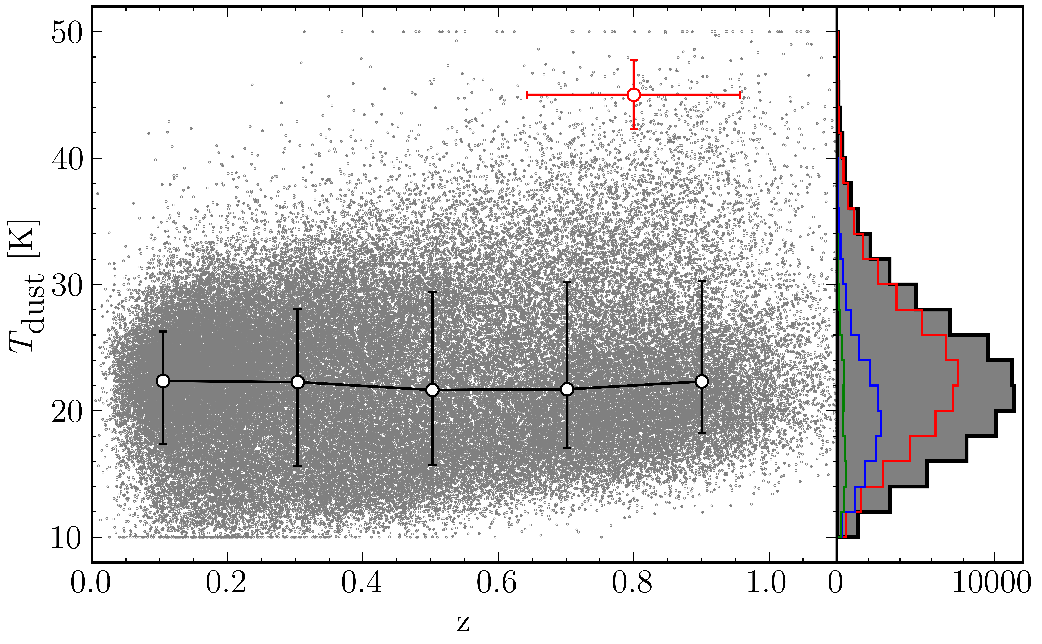
\includegraphics[width=0.8\columnwidth]{Figures/dust_temperatures.pdf}
	\caption[The distribution of dust temperatures as a function of redshift]{The dust temperature against redshift for galaxies in the SGP field. The red cross illustrates the typical $1\sigma$ error in the redshifts and dust temperatures. The black error bars represent the median dust temperature in each redshift bin, along with the $1\sigma$ range in the distribution ($16$th to $84$th percentiles). The righthand panel shows the histogram of dust temperatures for all galaxies (grey filled), galaxies with SNR $> 4$ in one band (red), in two bands (blue) and in three bands (green).}
	\label{fig:dust_temperatures}
\end{figure}

In the next section we shall start from the assumption that the dust spectrum of all galaxies in our sample can be approximated by an SED with a characteristic dust temperature of $20\,$K when deriving the DMF (e.g. \citealt{Vlahakis_2005}). This knowledge is required for certain methods used to derive a binned DMF in $M_{\textrm{dust}}-z$ space as they rely on knowing the shape of the SED to apply appropriate K-corrections in each bin. As we shall explain later, some methods for calculating binned functions allow for each galaxy to use its own dust spectrum rather than a global SED to compute the required K-corrections. We shall discuss how this impacts our DMF in later sections.

We calculate dust masses from monochromatic rest frame luminosities, which we derive from the K-corrected observed flux densities at $250\,\mu$m. We translate the $250\,\mu$m flux densities of the SGP galaxies into monochromatic luminosities using

\begin{equation}
    L_{250} = \frac{4\pi D_L^2 S_{250}K}{(1+z)},
\label{eq:monohromatic_luminosities}
\end{equation}

\noindent where $L_{250}$ is in units of W Hz$^{-1}$, $D_L$ is the luminosity distance, $S_{250}$ is the observed flux density at $250\,\mu$m and $K$ is the K-correction that allows us to define a rest frame quantity at $250\,\mu$m in terms of the observed frame at the same wavelength, given by

\begin{equation}
    K = \frac{S_{250}^{K}}{S_{250}^{\textrm{obs}}} = \Bigg(\frac{\nu_{K}}{\nu_{\textrm{obs}}}\Bigg)^{3+\beta}\frac{e^{(h\nu_{\textrm{obs}}/kT)} - 1}{e^{(h\nu_{K}/kT)} - 1},
\label{eq:k_correction}
\end{equation}

\noindent where $\nu_{K} = \nu_{\textrm{obs}}(1+z)$ and $T$ and $\beta$ are the dust temperature and emissivity index describing the SED. 

Let us briefly consider a galaxy at the edge of our redshift range, $z \sim 1$. The factor $K$ allows us to convert $S_{250}^{\textrm{obs}}$, the emission radiated at $250\,\mu$m ($1.2\,$THz) and observed at $125\,\mu$m ($2.4\,$THz) to $S_{250}^{K}$, the $250\,\mu$m flux density in the galaxy's rest frame. The monochromatic luminosity at $250\,\mu$m is then converted to a dust mass using

\begin{equation}
    M_{\textrm{dust}} = \frac{L_{250}}{4\pi\kappa_{250}B(\nu_{250}, T)},
\label{fig:dust_mass}
\end{equation}

\noindent where $\kappa_{250}$ is the dust mass absorption coefficient at $250\,\mu$m. The dust mass absoprtion coefficient is an amalgamation of terms including the efficiency with which the dust grains emit in reference to a perfect blackbody, the size of the dust grains and their mass volume density. For this reason, the value of $\kappa_\nu$ is highly uncertain with a wide range of values spanning multiple orders of magnitude being presented in the literature (\citealt{Clark_2019}). A commonly used value is $0.077\,$m$^2$kg$^{-1}$ at $850\,\mu$m (\citealt{Dunne_2000, daCunha_2008, Dunne_2011}) which represents a theoretical value lying between the expected value for graphite and silicate dust grains (\citealt{Draine_1984}). Assuming $\beta = 2$ we scale this value to $250\,\mu$m such that $\kappa_{250} = 0.89\,$m$^2$kg$^{-1}$.

\section{Sources of Incompleteness}

An important issue to consider when deriving our DMF is the completeness of our \textit{Herschel} survey and how we may account for missing galaxies when estimating the space-density of objects. In the following sections we outline the methods we use to estimate the incompleteness of our sample and thus the completeness correction factors we apply to our SGP catalogue, in order to account for sources we either do not observe or do not retain from the LR method described earlier. Each object in our SGP sample will be multiplied by correction factors that compensate for the number of times we might expect to observe this type of galaxy, based on the number of missing \textit{Herschel} sources and sources without a near-IR identification.

\subsection{\textit{Herschel} Catalogue Incompleteness}

The first correction factor is a direct result of the source extraction process used to create the \textit{Herschel} catalogues from the far-IR images. Due to source confusion these catalogues are incomplete as we approach the flux limit of the survey. To determine the completeness of the H-ATLAS catalogues, \citealt{Valiante_2016} used a catalogue of simulated sources embedded in real H-ATLAS maps to predict the efficiency of the \texttt{MADX} algorithm in recovering the sources. The completeness is shown as a function of the measured $250\,\mu$m flux density in Figure \ref{fig:submm_completeness} and is listed in Table \ref{tab:submm_completeness_table} along with the correction factors, $c_{\textrm{far-IR}}$, defined as the reciprocal of the completeness. We use an interpolated version of this table when applying the correction factors to our SGP galaxies. Unsurprisingly, the highest correction factors are found as we approach the flux limits of the survey where confusion noise dominates and the likelihood of lost sources rises.

\begin{table}
    \centering
    \begin{tabular}{p{5cm}|p{2.5cm}|p{2.5cm}}
        \hline
        \hline
        $250\,\mu$m Flux Density [mJy] & Completeness & $c_{\textrm{far-IR}}$ \\
        \hline
        \hline
        20.0 & 0.541 & 1.849 \\
        26.5 & 0.762 & 1.313 \\
        35.1 & 0.903 & 1.107 \\
        46.4 & 0.969 & 1.032 \\
        61.5 & 0.989 & 1.011 \\
        81.4 & 0.993 & 1.007 \\
        107.7 & 0.997 & 1.003 \\
        142.6 & 0.997 & 1.003 \\
        188.8 & 0.997 & 1.003 \\
        250.0 & 0.999 & 1.001 \\
        \hline
    \end{tabular}
    \caption[Far-IR catalogue completeness as a function of $250\,\mu$m flux density]{The far-IR completeness and corresponding correction factors as a function of the measured flux density.}
    \label{tab:submm_completeness_table}
\end{table}

\subsection{Reliable ID Incompleteness}

The second correction function arises from our inability to match all the \textit{Herschel} sources, for which we have observed a candidate on the VIKING image, with a high reliability counterpart. The unmatched sources are largely the result of large positional uncertainties, the possibility of coincident background objects and multiple systems where the sources are associated with each other but treated independently by the LR method.

In its simplest form, the completeness of our reliable sample is defined as the redshift distribution of our IDs divided by the true redshift distribution of \textit{Herschel} counterparts, scaled to the number of sources for which we observe a nearby VIKING counterpart; $C_{\textrm{id}} = n_{\textrm{reliable}}(z)/n_{\textrm{real, scaled}}(z)$. This second term is closely related to the probability distribution of true counterparts as a function of redshift, $q(z)$, much like the true counterparts distribution we derived as a function of $K_s$-band magnitude in the previous Chapter. Using the same formalism as Equation \ref{eq:true_counterparts_distribution}, we define the denominator as

\begin{equation}
    n_{\textrm{real, scaled}} = q(z)\times N_{\textrm{250\,\micron}} = \frac{n_{\textrm{real}}(z)}{\sum_{z_i}n_{\textrm{real}}(z_i)}\times QN_{\textrm{250\,\micron}},
    \label{eq:n_real_scaled}
\end{equation}

\noindent where $n_{\textrm{real}}(z)$ is the redshift distribution of true counterparts (recall Equation \ref{eq:real_distribution}) and $N_{\textrm{250\,\micron}}$ is the number of $250\,\mu$m \textit{Herschel} positions. As previously, the required correction functions are the reciprocal of the completeness. When we derived the $q(m)$ distribution in Section \ref{sec:true_counterparts_distribution} we noted that the distribution is normalized such that the integral of $q(m)$ up to the limiting magnitude of the VIKING survey is equal to the probability that the source is detected ($\int^{m_\textrm{lim}} q(m) dm = Q$). As an extension of this normalization, we recognize that the integral of the ID redshift distribution multiplied by the correction factors should give the total number of sources with observable counterparts (i.e. $\int_z c_{\textrm{id}} n_{\textrm{reliable}}(z) dz = QN_{\textrm{250\,\micron}}$, where $c_{\textrm{id}}$ are the correction factors given by $1/C_{\textrm{id}}$).

The ID completeness as a function of redshift is listed in Table \ref{tab:id_completeness_table} and illustrated in Figure \ref{fig:id_completeness} alongside the completeness functions from the SDP (\citealt{Smith_2011}), GAMA9 field (\citealt{Fleuren_2012}) and NGP (\citealt{Bourne_2016}). The average correction factor per source in the SGP is approximately two. Near the median redshift of the distribution ($z \sim 0.5$) the completeness is lower in the SGP than in other fields, though we note that we do not include spectroscopic redshifts, which might lower our completeness. The general trend for all H-ATLAS studies is a steady decline from $\sim 100\%$ completeness at $z = 0$ to a minimum at $z \sim 0.5 - 0.7$ followed by a rise at higher redshifts. The decrease towards $z = 0.5$ might be a result of a fixed search radius corresponding to a greater physical scale at larger cosmological distances. This would result in a greater probability of observing spurious counterparts that decrease the ID rate. Presently, we are not sure why the ID completeness rises again at higher redshifts, but one possible explanation is the greater probability of lensing events along the line of sight 

\begin{table}
    \centering
    \begin{tabular}{p{4.5cm}|p{2.5cm}|p{2.5cm}}
        \hline
        \hline
        Redshift & Completeness & $c_{\textrm{id}}$ \\
        \hline
        \hline
        0.05 & 0.984 & 1.016 \\
        0.15 & 0.881 & 1.135 \\
        0.25 & 0.713 & 1.403 \\
        0.35 & 0.542 & 1.844 \\
        0.45 & 0.432 & 2.313 \\
        0.55 & 0.387 & 2.581 \\
        0.65 & 0.372 & 2.685 \\
        0.75 & 0.360 & 2.776 \\
        0.85 & 0.392 & 2.552 \\
        0.95 & 0.422 & 2.369 \\
        \hline
    \end{tabular}
    \caption[ID completeness as a function of redshift]{The counterpart ID completeness and corresponding correction factors as a function of redshift.}
    \label{tab:id_completeness_table}
\end{table}

\begin{figure}
	\centering
	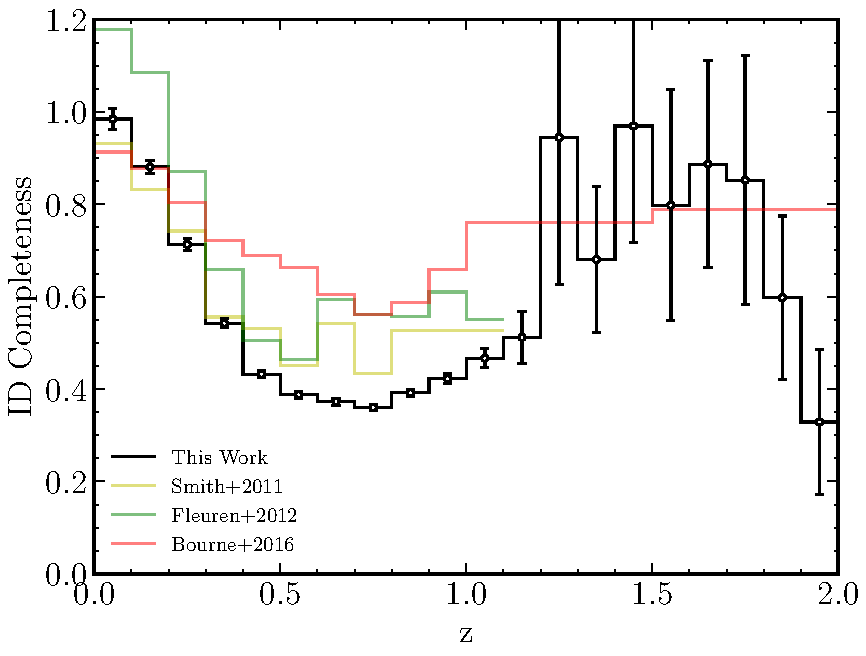
\includegraphics[width=0.8\columnwidth]{Figures/id_completeness.pdf}
	\caption[Completeness of our reliable SGP sample as a function of redshift]{The completeness of our $R > 0.8$ SGP sample as a function of redshift (black error bars), calculated using $n_{\textrm{reliable}}(z)/n_{\textrm{real, scaled}}$ where $n_{\textrm{real, scaled}}(z)$ is given by Equation \ref{eq:n_real_scaled}. Completeness functions from other H-ATLAS studies; \citealt{Smith_2011}, \citealt{Fleuren_2012} and \citealt{Bourne_2016}, are shown as yellow, green and red lines, respectively.}
	\label{fig:id_completeness}
\end{figure}

\section{Estimators of the Binned Dust Mass Function}
\label{sec:dmf_estimators}

The dust mass function, $\phi(M_{\textrm{dust}})$, represents the space density of galaxies as a function of dust mass, which in its differential form is given as the number of galaxies per unit comoving volume per unit dust mass interval

\begin{equation}
    \phi(M_{\textrm{dust}}, z) = \frac{d^2N}{dV dM_{\textrm{dust}}},
\label{eq:differential_phi}
\end{equation}

\noindent where $N$ is the number of galaxies with dust mass $M_{\textrm{dust}}$ observed in the comoving volume $V$ at redshift $z$. In this section we outline two methods of calculating the binned dust mass function; the ubiquitously used $1/V_{\textrm{max}}$ method \mbox{(\citealt{Schmidt_1968, Felten_1976, Avni_1980})} and the approximate method, $\phi_{\textrm{est}}$, proposed by \citealt{Page_2000}. Alternative parametric methods (e.g. the maximum-likelihood method of \citealt{Marshall_1983}) allow us to explore the entire $M_{\textrm{dust}} - z$ space, including regions that are not covered by observational data, and allow us to produce continuous functions for $\phi(M_{\textrm{dust}}, z)$. Although it is well established that the dust mass function can be parameterized in the form of a Schechter function (\citealt{Press_1974, Schechter_1976}), it is not obvious how this function evolves with redshift and which functional form should be used for this evolution. For this reason, we prefer to use binned, non-parametric methods and empirically study the redshift evolution of the DMF.

\subsection{The $1/V_{\textrm{max}}$ Method}

The prevalent use of the $1/V_{\textrm{max}}$ method stems from our need to overcome the Malmquist bias (\citealt{Eddington_1914, Malmquist_1922}) that causes selection biases in flux density limited samples. Malmquist bias refers to the tendency for flux-limited samples to be increasingly dominated by more luminous sources with increasing cosmological distance. As a result, more luminous objects are detected in larger volumes than less luminous objects, which needs to be accounted for in our space-density calculations. The $1/V_{\textrm{max}}$ method corrects for this bias by weighting each galaxy according to the maximum comoving volume in which it can be observed by the survey. The number density of galaxies in a given dust mass-redshift bin ($\Delta M_{\textrm{dust}} \Delta z$) is approximately given by the sum of the reciprocal maximum comoving volume for all galaxies in this bin

\begin{equation}
    \frac{dN}{dV} \sim \sum_{i=1}^N \frac{1}{V_{\textrm{max,i}}(M_{\textrm{dust,i}},z)},
\label{eq:number_density_1/v_method}
\end{equation}

\noindent where $V_{\textrm{max,i}}$ is the maximum comoving volume in which the $i$th galaxy in this bin could be detected by the survey. The volume is calculated according to

\begin{align}
    V_{\textrm{max},i}(M_{\textrm{dust,i}},z) &= \int^{\scriptscriptstyle \textrm{survey}} \int_{\scriptscriptstyle z_1}^{\scriptscriptstyle \textrm{min}[z_2, z(M_{\textrm{dust,i}},S_{\textrm{lim}})]} \frac{dV}{dz} dz d\Omega \nonumber \\
    &= \int^{\scriptscriptstyle \textrm{survey}} \int_{\scriptscriptstyle z_1}^{\scriptscriptstyle \textrm{min}[z_2, z(M_{\textrm{dust,i}},S_{\textrm{lim}})]} D_H \frac{(1+z)^2 D_A^2}{E(z)} dz d\Omega
\label{eq:volume_1/v_method}
\end{align}

\noindent where $\frac{dV}{dz}$ is the differential comoving volume given in the following line in terms of the Hubble distance, $D_H$, the angular diameter distance, $D_A$, and the dimensionless Hubble parameter, $E(z)$. The integration over redshift has limits from the bottom redshift of the bin, $z_1$, to either the upper edge of the bin, $z_2$, or the redshift beyond which the galaxy with dust mass $M_{\textrm{dust},i}$ would not be observed, whichever is smallest. A graphical illustration of the dust mass-volume space available to a galaxy with a dust mass $M_{\textrm{dust},i}$ is presented in the left-hand panel of Figure \ref{fig:volume_comparison}.

The binned dust mass function using this method is then defined by dividing the number density by the dust mass bin width (which we define in terms of logarithmic dust mass)

\begin{equation}
    \phi_{1/V}(M_{\textrm{dust}},z) = \frac{1}{\Delta \textrm{log}_{10}(M_{\textrm{dust}})} \sum_{i=1}^N \frac{1}{V_{\textrm{max,i}}(M_{\textrm{dust,i}},z)}.
\label{eq:phi_1/v_method}
\end{equation}

To account for the incompleteness of the sample, we include the correction factors we derived in the previous section in the following way

\begin{equation}
    \phi_{1/V}(M_{\textrm{dust}},z) = \frac{1}{\Delta \textrm{log}_{10}(M_{\textrm{dust}})} \sum_{i=1}^N \frac{c_{\scriptscriptstyle \textrm{far-IR}} c_{\scriptscriptstyle \textrm{id}}}{V_{\textrm{max,i}}(M_{\textrm{dust,i}},z)}.
\label{eq:phi_1/v_method}
\end{equation}

While this method suitably deals with Malmquist bias and does not require an a-priori analytic form, it can produce unwanted artefacts when applied to flux-limited samples. The problem arises when we have an uncertain estimate of the $250\,\mu$m flux density, a result of the confused \textit{Herschel} images, leading to large variance in the calculation of $V_{\textrm{max,i}}(M_{\textrm{dust,i}},z)$. An alternative method that better handles the accessible volume calculation for objects close to the flux limit of the survey is the method of \citealt{Page_2000} (hereafter PC00).

\subsection{The Page and Carrera Method}

In the $1/V_{\textrm{max}}$ method we assumed that the accessible comoving volume in which a galaxy could have been detected by the survey is constant across all dust masses in a given $M_{\textrm{dust}} - z$ bin.

The PC00 method, however, has the advantage that the comoving volume is defined from the average value for all dust masses in the interval $\Delta M_{\textrm{dust}}$. By taking an average over the dust mass interval, we do not require the, potentially very uncertain, measured flux density values for each source in order to calculate the accessible volumes. In a similar fashion as before, the number density of galaxies is approximately given by the sum of all galaxies in the bin divided by the average accessible volume, 

\begin{equation}
    \frac{dN}{dV} \sim \frac{\sum_{i=1}^N 1}{V_{\textrm{max,av}}(M_{\textrm{dust}},z)},
\label{eq:number_density_pc00_method}
\end{equation}

\noindent where $V_{\textrm{max,av}}$ now represents an average volume for all galaxies in the bin. This volume is averaged over all dust masses in the range $M_{\textrm{dust, 1}} < M_{\textrm{dust}} < M_{\textrm{dust, 2}}$ following

\begin{multline}
    V_{\textrm{max,av}}(M_{\textrm{dust}},z) = \frac{1}{\Delta \textrm{log}_{10}(M_\textrm{dust})}\int_{\scriptscriptstyle M_{\textrm{dust,1}}}^{\scriptscriptstyle M_{\textrm{dust,2}}} \int^{\scriptscriptstyle \textrm{survey}} \int_{\scriptscriptstyle z_1}^{\scriptscriptstyle \textrm{min}[z_2, z(M_{\textrm{dust}},S_{\textrm{lim}})]} \\ D_H \frac{(1+z)^2 D_A^2}{E(z)} dz d\Omega d\textrm{log}_{10}(M_\textrm{dust}),
\label{eq:volume_pc00_method}
\end{multline}

\noindent which is akin to Equation \ref{eq:volume_1/v_method}, except we integrate over all dust masses and divide by the bin width. Crucially, this means that we are not dependent on any individual estimate of the dust mass, $M_{\textrm{dust,i}}$. The dust mass-volume space for an example bin is shown in the right-hand panel of Figure \ref{fig:volume_comparison}. In the same manner as before, the dust mass function is defined as the number density divided by the dust mass bin width:

\begin{align}
    \phi_{\textrm{est}}(M_{\textrm{dust}},z) &= \frac{1}{\Delta \textrm{log}_{10}(M_{\textrm{dust}})} \times \nonumber \\
    & \qquad \frac{\sum_{i=1}^N c_{\scriptscriptstyle \textrm{far-IR}} c_{\scriptscriptstyle \textrm{id}}}{\frac{1}{\Delta \textrm{log}_{10}(M_\textrm{dust})}\int_{\scriptscriptstyle M_{\textrm{dust,1}}}^{\scriptscriptstyle M_{\textrm{dust,2}}} \int^{\scriptscriptstyle \textrm{survey}} \int_{\scriptscriptstyle z_1}^{\scriptscriptstyle \textrm{min}[z_2, z(M_{\textrm{dust}},S_{\textrm{lim}})]} D_H \frac{(1+z)^2 D_A^2}{E(z)} dz d\Omega d\textrm{log}_{10}(M_\textrm{dust})} \nonumber \\
    &= \frac{\sum_{i=1}^N c_{\scriptscriptstyle \textrm{far-IR}} c_{\scriptscriptstyle \textrm{id}}}{\int_{\scriptscriptstyle M_{\textrm{dust,1}}}^{\scriptscriptstyle M_{\textrm{dust,2}}} \int^{\scriptscriptstyle \textrm{survey}} \int_{\scriptscriptstyle z_1}^{\scriptscriptstyle \textrm{min}[z_2, z(M_{\textrm{dust}},S_{\textrm{lim}})]} D_H \frac{(1+z)^2 D_A^2}{E(z)} dz d\Omega d\textrm{log}_{10}(M_\textrm{dust})}.
\label{eq:phi_pc00_method}
\end{align}

In the PC00 method as defined above, the accessible volume is calculated for each $M_{\textrm{dust}} - z$ bin assuming a global SED shape to translate the flux limit of the survey to a limiting dust mass at each redshift. This means that all galaxies in a bin are assumed to follow the same limiting $M_{\textrm{dust}} - z$ relationship. \citealt{Dunne_2011} present a modified version of the PC00 method that allows each galaxy to set its own limiting $M_{\textrm{dust}} - z$ relationship, allowing for a range of SEDs observed in each bin. In this form, each galaxy in the bin has an individual contribution to the dust mass function such that

\begin{equation}
    \phi_{\textrm{est, Dunne}}(M_{\textrm{dust}},z) = \sum_{i=1}^N \frac{c_{\scriptscriptstyle \textrm{far-IR}} c_{\scriptscriptstyle \textrm{id}}}{\int_{\scriptscriptstyle M_{\textrm{dust,1}}}^{\scriptscriptstyle M_{\textrm{dust,2}}} \int^{\scriptscriptstyle \textrm{survey}} \int_{\scriptscriptstyle z_1}^{\scriptscriptstyle \textrm{min}[z_2, z(M_{\textrm{dust}},S_{\textrm{lim,i}})]} D_H \frac{(1+z)^2 D_A^2}{E(z)} dz d\Omega d\textrm{log}_{10}(M_\textrm{dust})},
\label{eq:phi_pc00_dunne_method}
\end{equation}

\noindent where we see that the integration over redshift is now computed individually for each source. This has the added benefit of allowing a unique flux limit to be used for each galaxy $S_{\textrm{lim,i}}$, which is useful for surveys like H-ATLAS where source extraction is based on the SNR of the source rather than a single flux cut.

\subsection{Comparison of Estimators}

While the $1/V_{\textrm{max}}$ estimator is a perfectly adequate way of accounting for Malmquist bias, the PC00 method provides additional advantages for far-IR derived DMFs. Most importantly, the accessible volume is not dependent on the dust mass of any individual galaxy, which can have significant uncertainties due to flux boosting. Second, the two approaches give very different answers when calculating the accessible volume in underpopulated bins near the flux limit of the survey. Figure \ref{fig:volume_comparison} shows a comparison of the accessible volume calculation for an example $M_{\textrm{dust}} - z$ bin ($8 < \textrm{log}_{10}(M_\textrm{dust} [M_\odot]) < 8.25, 0.2 < z < 0.4$). In this example of an undersampled bin, the volume calculated from the $1/V_{\textrm{max}}$ method will typically be an overestimate of the true region of the dust mass-volume space that has been surveyed, leading to an underestimate of the DMF in the lowest mass bin of a given redshift slice. As a test of consistency, in bins where all objects are brighter than the flux limit of the survey, the volume estimates should yield the same result and we expect the DMFs to be identical.

\begin{figure}
	\centering
	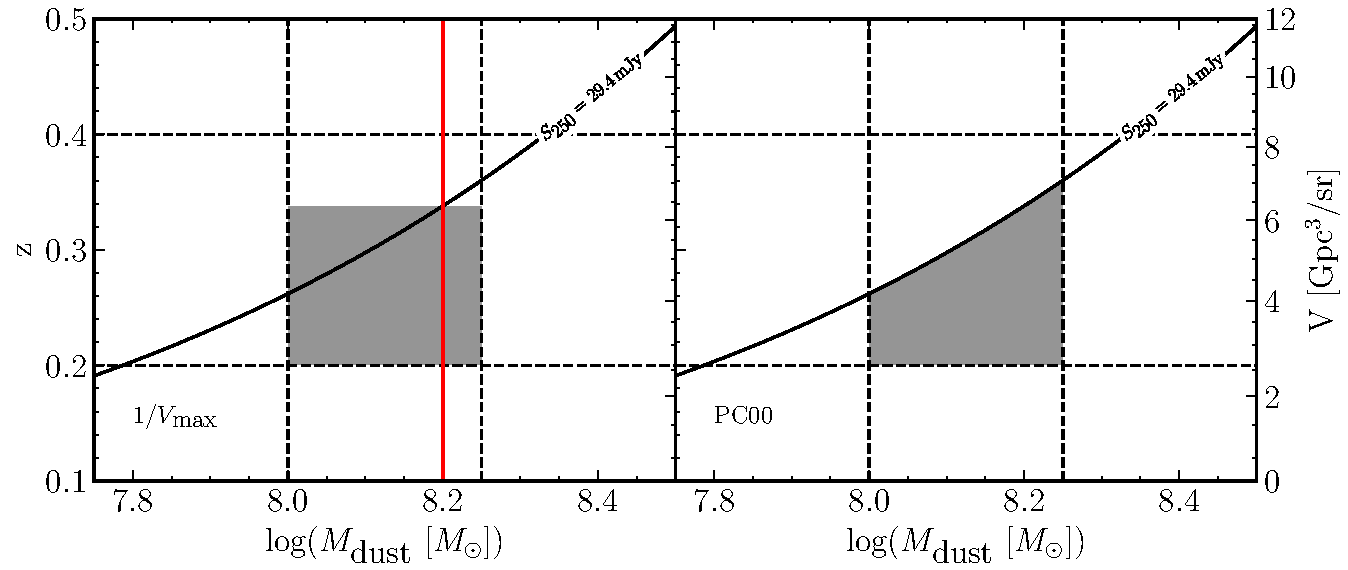
\includegraphics[width=\columnwidth]{Figures/volume_comparison.pdf}
	\caption[Example dust mass - redshift bin for the $1/V_{\textrm{max}}$ and PC00 methods]{An illustration of the accessible volume calculated in the $1/V_{\textrm{max}}$ (left panel) and PC00 methods (right panel), using Equations \ref{eq:volume_1/v_method} and \ref{eq:volume_pc00_method} respectively. Having defined an example dust mass - redshift bin ($8 < \textrm{log}(M_{\textrm{dust}} [M_{\odot}]) < 8.25$, $0.2 < z < 0.4$), the shaded areas in both panels represent the volume - dust mass space that is observable in a \textit{Herschel} survey with a limiting flux of $29.4\,$mJy at $250\,\mu$m. In the $1/V_{\textrm{max}}$ panel we have illustrated the volume as it would appear for an object with a dust mass of $8.2\,\textrm{log}(M_{\odot}$).}
	\label{fig:volume_comparison}
\end{figure}

\section{The Dust Mass Function from Galaxies in the SGP}
\label{sec:dmf_from_sgp}

We apply the three methods described above to the galaxies observed in the H-ATLAS SGP field. It is important to note that our sample is without spectroscopic redshifts and our dust masses are derived from sub-mm fluxes that are susceptible to flux boosting. The resulting scatter in the dust masses and redshifts could move galaxies between neighbouring bins. Given that the volume density is not uniform across bins and the survey is flux-limited, this introduces an Eddington bias (\citealt{Eddington_1913}) that broadens the DMF. For this reason, we model the errors as being formed in two parts. First, a Poissonian error that scales as $\sigma_{\phi,N} \propto \frac{1}{\sqrt{N}}$, where $N$ is the number of galaxies in each bin. The second error term is due to the spread in dust masses as a result of the large uncertainties on our photometric redshifts (see Section \ref{sec:phot_z_VIKING}). When measuring the DMF we run $1000$ Monte Carlo simulations in which we remeasure the DMF having perturbed the redshift of each galaxy according to a Gaussian distribution centered on the assumed redshift and with standard deviation equal to the error value. This gives us a 3D array ($M_{\textrm{dust}} - z - n$, where $n$ is the number of Monte Carlo interations) of $\phi$. We take the standard deviation along the $n$ axis, $\sigma_{\phi,z}^2$, and add this error in quadrature to the Poissonian error: $\sigma_\phi = \sqrt{\sigma_{\phi,N}^2 + \sigma_{\phi,z}^2}$.

Figure \ref{fig:dmf_methods} shows the DMFs derived using the PC00 (solid lines) and $1/V_{\textrm{max}}$ (dashed lines) methods for five redshift bins of width $0.2$, assuming a universal dust temperature of $20\,$K and dust emissivity index, $\beta = 2$. As a single SED shape is being assumed for all galaxies, we must also assume a single survey flux limit - which we take to be $29.4\,$mJy at $250\,\mu$m (\citealt{Valiante_2016}). As we predicted for bins that are entirely above the flux limit of the sample, the two estimators are equivalent. Also predicted earlier was the downturn observed in the lowest dust mass bin in most redshift slices.

The low-mass end of the DMF is typically described by a powerlaw with a gradient, $\alpha$, taking values between $-2$ and $-1$. In the lowest redshift bin, we observed dust masses small enough to constrain the value of $\alpha$, finding much flatter values than general consensus, suggesting that the number density of low redshift galaxies between dust masses of $\sim 10^{5.5}\,M_{\odot}$ and $\sim 10^{7.5}\,M_{\odot}$ is near constant. In light of previous H-ATLAS studies that do not predict this behaviour, we expect that this is not a physical trend but rather an indication of an incomplete sample at the lowest masses. Given we are not using spectroscopic redshifts, we are likely missing some of these galaxies in our sample. While we cannot rule out that the DMF has a low normalization at low dust masses, as is also seen in other studies such as \citealt{Dunne_2011}, from this point onwards we shall assume that our DMFs are accurate above $\sim 10^{7.5}\,M_{\odot}$ and use the results of \citealt{Beeston_2018} to fill in the low-mass regime. The \citealt{Beeston_2018} value of $\alpha$ was measured for low redshift galaxies, but without data to constrain this value at higher redshifts, we shall assume that this value is equally appropriate in all redshift bins.

Assuming these DMFs, we observe a clear evolution in the density of high dust mass galaxies increasing with redshift. The evolution with lookback time is evident in each redshift slice, but noticeably slows by the highest redshift bin. This may suggest that there is a point in time at redshifts $\gtrsim 0.8$ where the number density of the most massive galaxies peaks. As an extension to our $\phi_{\textrm{est}}$ prediction of the DMF, we would like to be able to use the estimator of \citealt{Dunne_2011} (Equation \ref{eq:phi_pc00_dunne_method}) in which we calculate the accessible volume individually for each source. The problem we face is that this requires knowing the dust temperatures of all galaxies in our sample. While we are able to constrain the dust temperatures for a subset of our sample, as shown in Figure \ref{fig:dust_temperatures}, we cannot depend on these sources alone without introducing another incompleteness to the sample. To avoid this problem we fit a single temperature modified blackbody to all galaxies, with bounds on the cold ISM dust temperature between $15$ and $25\,$K and with a fixed $\beta = 2$. This range of temperatures was chosen as it has been shown to be a suitable range of cold dust temperatures in galaxies (\citealt{Dunne_2001, daCunha_2008, Smith_2012b, Clark_2015, Beeston_2018}). Galaxies that have well constrained peaks in the dust emission are likely to have dust temperatures within this range, and those that have insufficient far-IR data to fit an isothermal model are assumed to take a median value of $20\,$K. Approximately $40\%$ of the galaxies in our sample have temperatures constrained between $15\,$K and $25\,$K; the remaining $\sim 60\%$ retain their $20\,$K assumption. We use this set of dust temperatures to calculate $\phi_{\textrm{est, Dunne}}$ assuming an individual survey flux limit for each source. The flux limit for each galaxy is based on a minimum SNR of four. As pointed out previously in \citealt{Dunne_2011}, this estimator is not equivalent to $\phi_{1/V}$, despite the contribution to $\phi$ being calculated for each galaxy individually in both methods. In the PC00 method we still calculate an average accessible volume for each $M_{\textrm{dust}} - z$ bin, but we now define the limiting dust mass -- redshift relationship for each source based on its own SED. This means we are more precise about the flux limit of the survey but do not depend on the uncertain dust mass estimates of the \textit{Herschel} galaxies. Our estimate of $\phi_{\textrm{est, Dunne}}$ is included in Figure \ref{fig:dmf_methods} (dotted lines). The \citealt{Dunne_2011} estimator of the DMF is broadly consistent with $\phi_{\textrm{est}}$, albeit with a wider distribution of dust masses due to the wider distribution of dust temperatures.

\begin{figure}
    \centering
    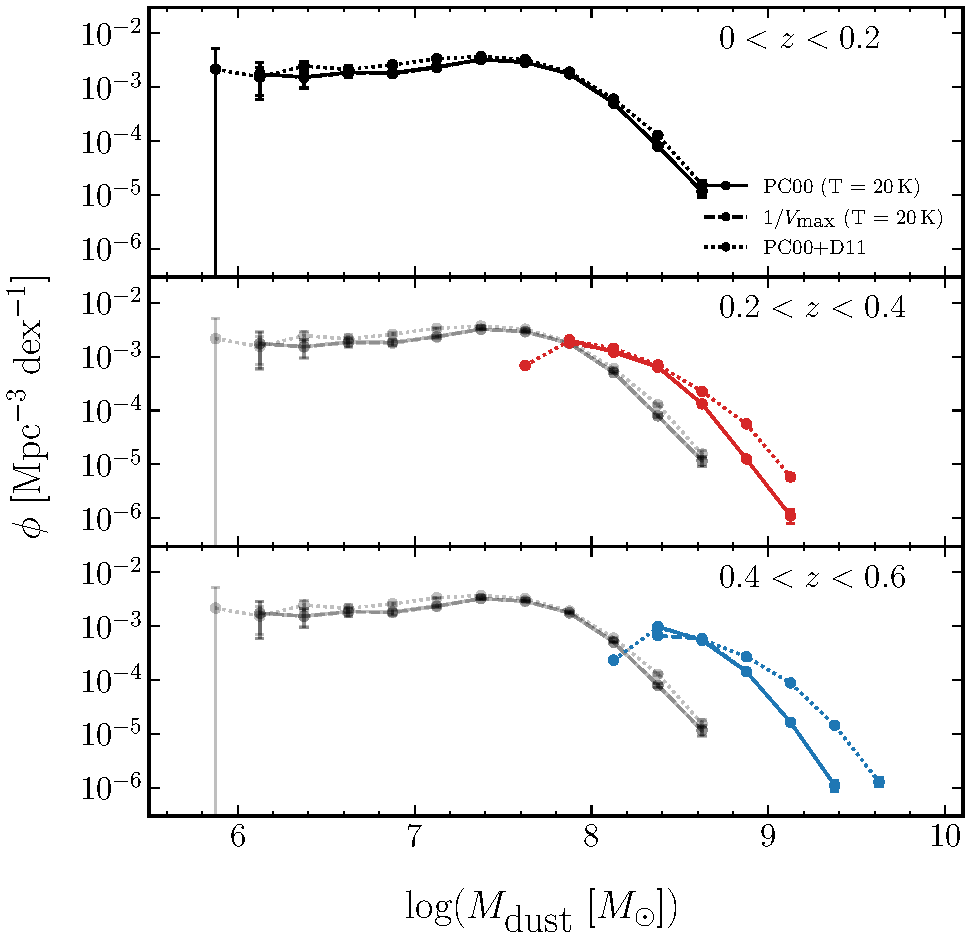
\includegraphics[width=\columnwidth]{Figures/Figure_3_4_part1.pdf}
    \caption[Dust mass functions derived from SGP galaxies]{The dust mass functions (DMFs) derived from SGP galaxies in five redshift bins of width $0.2$. The three methods described in Section \ref{sec:dmf_estimators}; the $1/V_{\textrm{max}}$, the Page and Carrera (\citealt{Page_2000}) and the Page and Carrera with the adaptation from \citealt{Dunne_2011} methods are illustrated as dashed lines, solid lines and dotted lines, respectively. In each panel the DMFs from the first redshift bin are replotted for comparison in grey. The final panel shows the DMFs from all redshift bins.}
	\label{fig:dmf_methods}
\end{figure}

\begin{figure}
    \ContinuedFloat
    \centering
    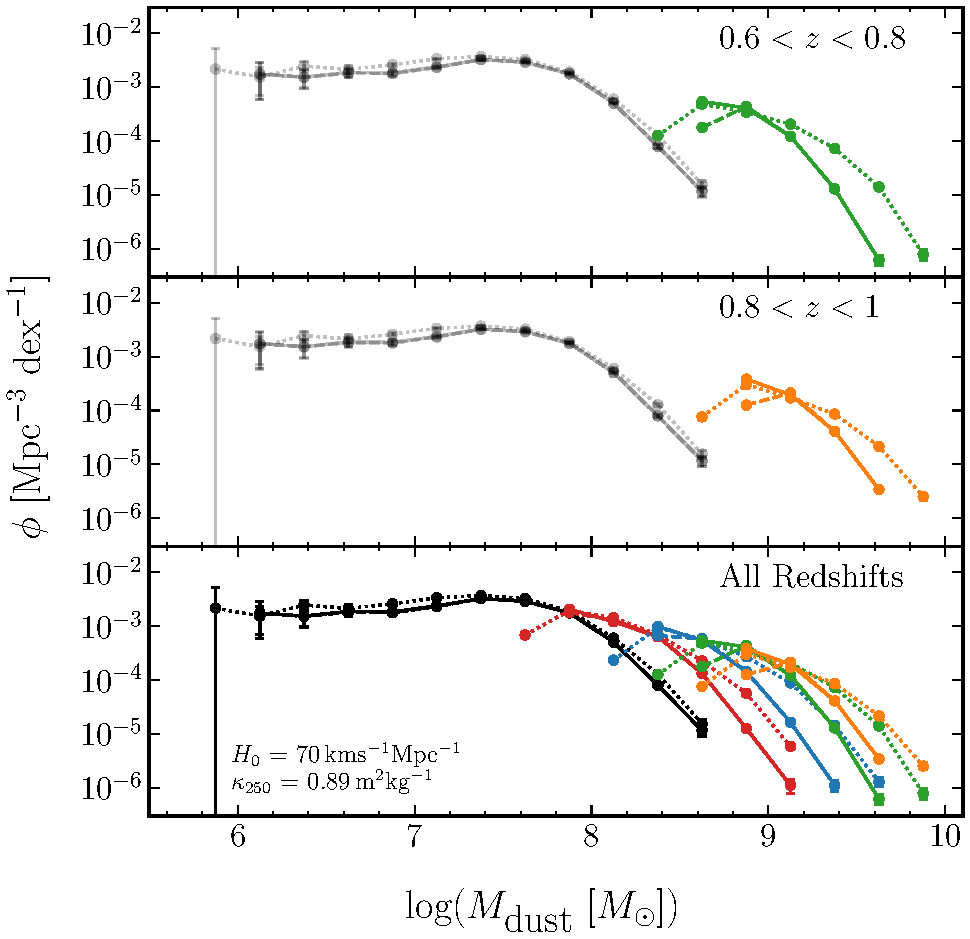
\includegraphics[width=\columnwidth]{Figures/Figure_3_4_part2.pdf}
    \caption{Continued.}
\end{figure}

\section{The Evolution in the Dust Content of SGP Galaxies}

In this section, we shall use the results of our two PC00 estimated DMFs to quantify the redshift evolution of dust mass in SGP galaixes. This is achieved in two ways: first by fitting Schechter functions to our DMFs and assessing the evolution in the Schechter parameters, and secondly, by calculating the dust mass density contained within galaxies at different epochs.

\subsection{Schechter Functions}
\label{sec:schechter_functions}

Luminosity functions, and by extension dust mass functions, are often modelled with analytical forms such as broken power laws or Schechter functions. The Schechter function takes the form

\begin{equation}
    \phi(M) dM = \phi^* (M/M^*)^\alpha e^{(-M/M^*)}\frac{dM}{M^*}
    \label{eq:schechter_function}
\end{equation}

\noindent in terms of mass, where $M^*$ is the characteristic dust mass where we transition from a powerlaw to an exponential tail, and $\alpha$ is the exponent of the low mass powerlaw. The normalization is defined by $\phi^*$ which corresponds to the number density of galaxies at mass $M^*$. We can convert the Schechter function to logarithmic form using the fact that $\phi(\textrm{log}(M)) = \textrm{ln}(10)M\phi(M)$ such that

\begin{equation}
    \phi(\textrm{log}(M)) d\textrm{log}(M) = \textrm{ln}(10)\phi^* e^{-10^{\textrm{log}(M)-\textrm{log}(M^*)}}\times \Bigg(10^{\textrm{log}(M)-\textrm{log}(M^*)}\Bigg)^{\alpha+1} d\textrm{log}(M).
    \label{eq:schechter_function_log}
\end{equation}

We incorporate the factor $\textrm{ln}(10)$ into our definition of $\phi^*$ such that $\phi^*$ has units of Mpc$^{-3}$dex$^{-1}$. Given the incompleteness of the lowest mass bins at high redshifts, it is common to fit the three Schechter parameters ($\phi^*$, $M^*$ and $\alpha$) for the first redshift bin and make the assumption that the value of $\alpha$ does not vary with redshift. Due to our sample incompleteness at low dust masses even in the lowest redshift slice, we fix our value of $\alpha$ to the \citealt{Beeston_2018} value of $-1.22$ throughout, and only consider values greater than $10^{7.5}\,M_{\textrm{dust}}$ in our fitting.

Figure \ref{fig:dmf_schechter} shows the best fit Schechter functions to our $\phi_{\textrm{est}}$ (solid lines, filled circles) and $\phi_{\textrm{est, Dunne}}$ (dotted lines, open circles) DMFs. The fitting parameters are listed in Table \ref{tab:schechter_parameters}. Included in Figure \ref{fig:dmf_schechter} are the studies of \citealt{Vlahakis_2005}, \citealt{Dunne_2011}, \citealt{Beeston_2018} and \citealt{Pozzi_2020}. For a direct comparison between all works we have scaled the DMFs in the literature to the same cosmology ($\Omega_m = 0.3$, $\Omega_\Lambda = 0.7$ and $H_0 = 70\,$km s$^{-1}$Mpc$^{-1}$) and dust mass absorption coefficient ($\kappa_{250} = 0.89\,$m$^{2}$kg$^{-1}$).

\begin{figure}
	\centering
	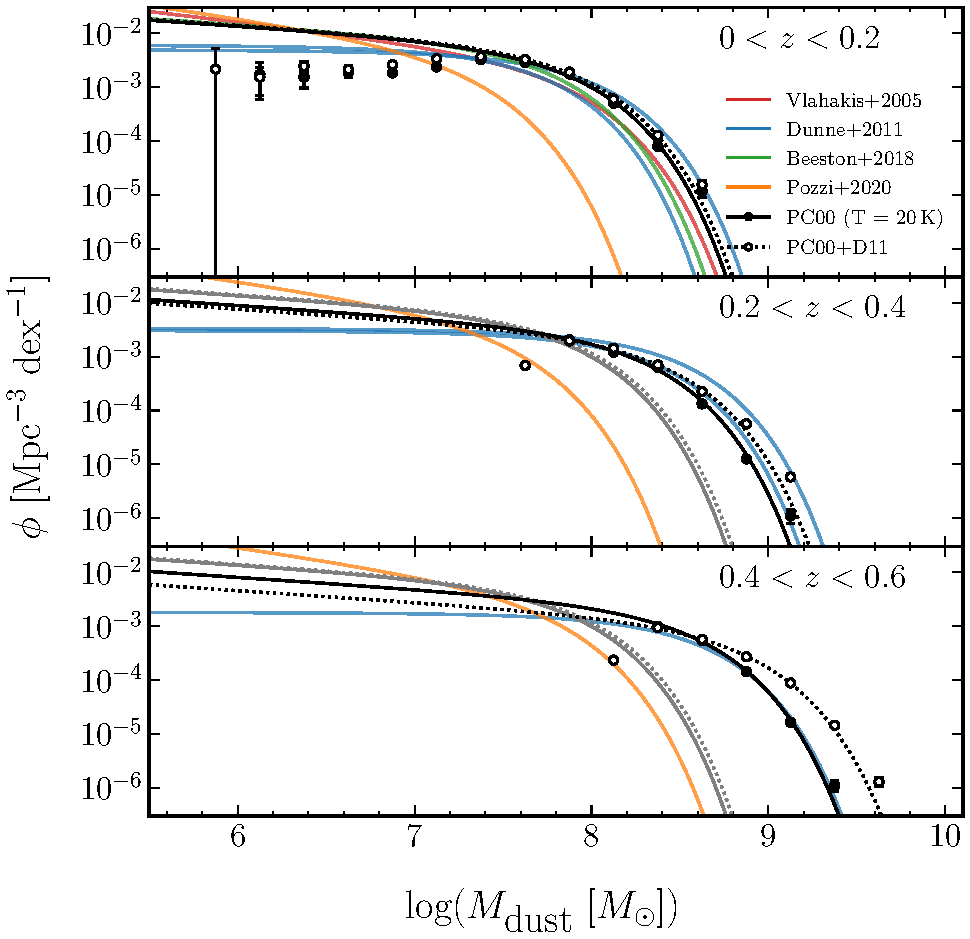
\includegraphics[width=\columnwidth]{Figures/Figure_3_5_part1.pdf}
    \caption[Schechter functions derived from the SGP DMFs alongside relevant studies]{The dust mass functions as presented in Figure \ref{fig:dmf_methods} (excluding the $1/V_{\textrm{max}}$ estimate), where the lines have been replaced with the best fitting Schechter functions (Equation \ref{eq:schechter_function_log}). The red, blue, green and orange lines represent the DMFs from \citealt{Vlahakis_2005}, \citealt{Dunne_2011}, \citealt{Beeston_2018} and \citealt{Pozzi_2020} respectively. The final panel shows the SGP DMFs from all redshift bins. The colour scales from the light to dark with increasing redshift.}
	\label{fig:dmf_schechter}
\end{figure}

\begin{figure}
    \ContinuedFloat
    \centering
    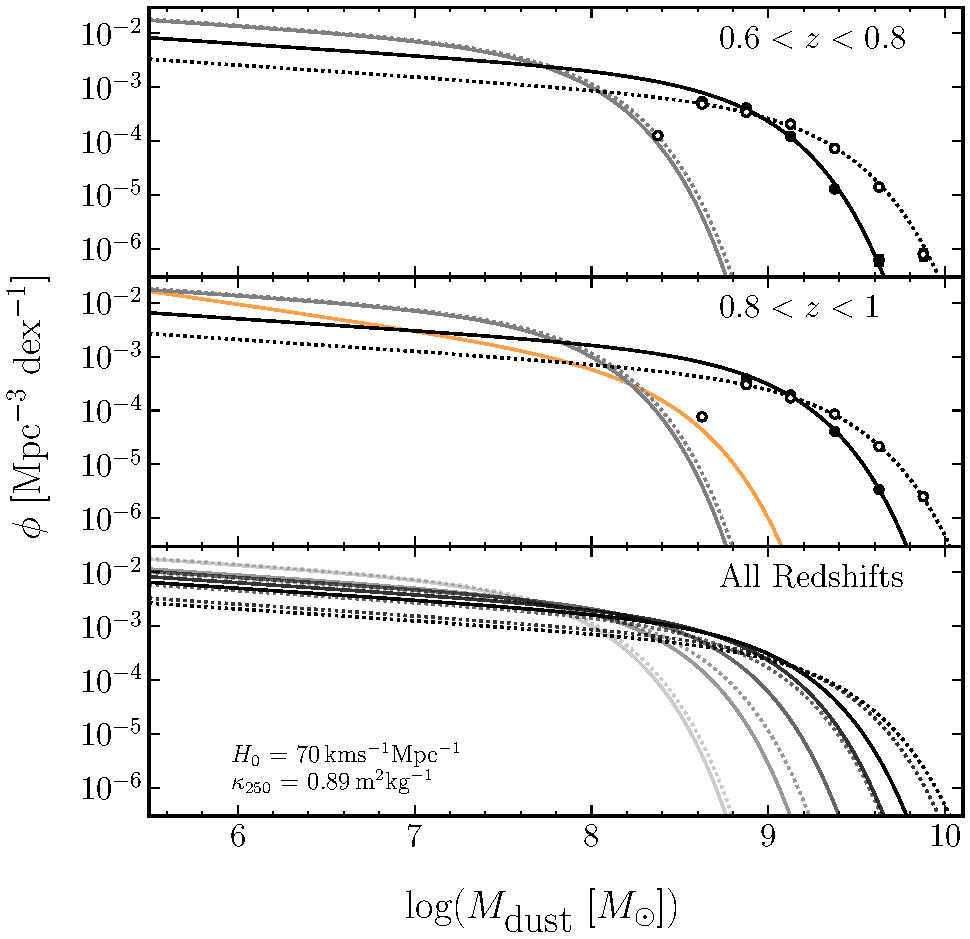
\includegraphics[width=\columnwidth]{Figures/Figure_3_5_part2.pdf}
    \caption{Continued.}
\end{figure}

\begin{table}
    \centering
    \begin{tabular}{p{1.75cm}|p{2.5cm}|p{2cm}|p{3.25cm}|p{1.25cm}|p{2cm}}
        \hline
        \hline
        Method & Redshift & log($M_{\textrm{dust}}^*$) & log($\phi^*$) & $\alpha$ & $\rho_{\textrm{dust}} (\times10^5)$ \\
        & & [log($M_{\odot}$)] & [log(Mpc$^{-3}$dex$^{-1}$)] & & [$M_{\odot}$Mpc$^{-3}$] \\
        \hline
        \hline
        \multirow{5}{*}{$\phi_{\textrm{est}}$} & 0 < z < 0.2 & $7.791^{+0.007}_{-0.007}$ & $-2.256^{+0.010}_{-0.011}$ & $-1.22$ & $1.770^{+0.051}_{-0.050}$ \\
        & 0.2 < z < 0.4 & $8.183^{+0.004}_{-0.005}$ & $-2.528^{+0.008}_{-0.008}$ & $-1.22$ & $2.331^{+0.048}_{-0.048}$ \\
        & 0.4 < z < 0.6 & $8.468^{+0.005}_{-0.005}$ & $-2.629^{+0.010}_{-0.010}$ & $-1.22$ & $3.560^{+0.088}_{-0.087}$ \\
        & 0.6 < z < 0.8 & $8.745^{+0.004}_{-0.004}$ & $-2.801^{+0.009}_{-0.009}$ & $-1.22$ & $4.542^{+0.104}_{-0.101}$ \\
        & 0.8 < z < 1 & $8.890^{+0.005}_{-0.005}$ & $-2.930^{+0.012}_{-0.012}$ & $-1.22$ & $4.695^{+0.139}_{-0.136}$ \\
        \hline
        \multirow{5}{*}{$\phi_{\textrm{est, Dunne}}$} & 0 < z < 0.2 & $7.827^{+0.007}_{-0.007}$ & $-2.249^{+0.010}_{-0.010}$ & $-1.22$ & $1.952^{+0.054}_{-0.053}$ \\
        & 0.2 < z < 0.4 & $8.305^{+0.004}_{-0.004}$ & $-2.628^{+0.006}_{-0.006}$ & $-1.22$ & $2.451^{+0.041}_{-0.040}$ \\
        & 0.4 < z < 0.6 & $8.747^{+0.005}_{-0.005}$ & $-2.943^{+0.006}_{-0.006}$ & $-1.22$ & $3.288^{+0.059}_{-0.059}$ \\
        & 0.6 < z < 0.8 & $9.117^{+0.003}_{-0.003}$ & $-3.277^{+0.003}_{-0.003}$ & $-1.22$ & $3.570^{+0.039}_{-0.039}$ \\
        & 0.8 < z < 1 & $9.195^{+0.004}_{-0.004}$ & $-3.386^{+0.004}_{-0.004}$ & $-1.22$ & $3.323^{+0.044}_{-0.044}$ \\
        \hline
    \end{tabular}
    \caption[Best fitting Schechter parameters of our SGP DMFs in each redshift slice]{The best fitting Schechter parameters for each redshift slice. The parameter $\phi^*$ incorporates the factor \textrm{ln}(10) such that it has units of Mpc$^{-3}$dex$^{-1}$. The uncertainties in the Schechter parameters are taken from the $16$th to $84$th percentiles of the posterior distribution for each parameter. The rightmost column lists the dust mass densities as calculated using Equation \ref{eq:dust_mass_density}.}
    \label{tab:schechter_parameters}
\end{table}

The local DMFs ($z < 0.2$) are in good agreement except for the low mass normalization and the offset in dust mass with the study of \citealt{Pozzi_2020}. While it is hard to reconcile the low normalizations found by our study and \citealt{Dunne_2011} with other works in the literature without a full understanding of the completeness of the respective samples at low flux densities, the shift in dust mass observed by \citealt{Pozzi_2020} in all redshift bins can be understood by comparing the selection wavelengths of the samples and their sensitivity to dust temperature. As mentioned previously, estimating dust masses from long wavelength photometry is advantageous as the Rayleigh-Jeans (R-J) part of the Planck function is least sensitive to dust temperature and most sensitive to dust mass. In the R-J regime ($\lambda_{\textrm{rest}} \gg \frac{hc}{kT}$) the Planck function reduces to $B(\nu_{250}, T) = \frac{2\nu_{250}^{2}kT}{c^2}$ which means that in the optically thin and R-J regimes our dust masses are only linearly dependent on the dust temperature.

This work, as well as the studies of \citealt{Dunne_2011} and \citealt{Beeston_2018}, are based on samples of H-ATLAS sources which are primarily selected at $250\,\mu$m. In the rest frame of the highest redshift galaxies considered here, the selection wavelength is still expected to be on the long wavelength side of the peak in dust emission. Further, at $850\,\mu$m, the SLUGS study of \citealt{Vlahakis_2005} is securely on the R-J side of the SED at the low redshifts probed in the SCUBA-selected study. As a result, these studies are sensitive to thermal emission from dust with fairly cool temperatures which should probe most of the dust mass. The $160\,\mu$m selection wavelength of \citealt{Pozzi_2020} means that in the rest frame this study probes different parts of the dust spectrum, crossing the peak to shorter wavelengths at $z \sim 0.5$. As we approach the peak of the dust SED an estimate of the dust mass becomes increasingly dependent on the measurement of the dust temperature - an effect that should also be noted when making conclusions from the highest redshift bins in our study. This is not to say that any study is inaccurate, but rather suggests that comparing studies with samples selected at different wavelengths may differ significantly, particularly if their dust temperatures are very different. It is also worth pointing out that there is a clear offset from the \citealt{Pozzi_2020} DMF even at $0 < z < 0.2$, where this effect is the least impactful, and therefore is not fully explained by this argument.

\subsection{Evolution of the Dust Mass Function}

To quantify the evolution we observe in dust masses of SGP galaxies, we can illustrate the variation in the characteristic dust mass and density in each redshift slice as obtained from our best fitting Schechter functions. Figure \ref{fig:dmf_schechter_parameters} shows the distribution of $\phi^*$ and $M_{\textrm{dust}}^*$ for our $\phi_{\textrm{est}}$ and $\phi_{\textrm{est, Dunne}}$ DMFs, as well as the studies considered in Figure \ref{fig:dmf_schechter}. We observe a strong evolution in the characteristic dust mass $M_{\textrm{dust}}^*$ with redshift, suggesting that galaxies were dustier at higher redshift. The density $\phi^*$ appears to decrease with redshift, but this is dependent on how well we account for the incompleteness in the sample. The characteristic dust mass evolves from $M_{\textrm{dust}}^* = 6.18\substack{+0.10\\-0.10}\times10^7\,M_{\odot}$ at $z < 0.2$ to $M_{\textrm{dust}}^* = 7.76\substack{+0.10\\-0.09}\times10^8\,M_{\odot}$ at $z = 0.8 - 1$, assuming a universal dust temperature of $20\,$K, suggesting a factor of $\sim 13$ in dust mass between the highest and lowest redshift bins. If we allow the $\sim 40\%$ of galaxies with well constrained dust temperatures to define their own K-corrections, then we observe a much steeper evolution from $M_{\textrm{dust}}^* = 6.71\substack{+0.10\\-0.10}\times10^7\,M_{\odot}$ to $M_{\textrm{dust}}^* = 1.57\substack{+0.01\\-0.02}\times10^9\,M_{\odot}$ over the same time period. This implies a factor increase twice as large compared to our $T_{\textrm{dust}} = 20\,$K DMF.

\begin{figure}
	\centering
	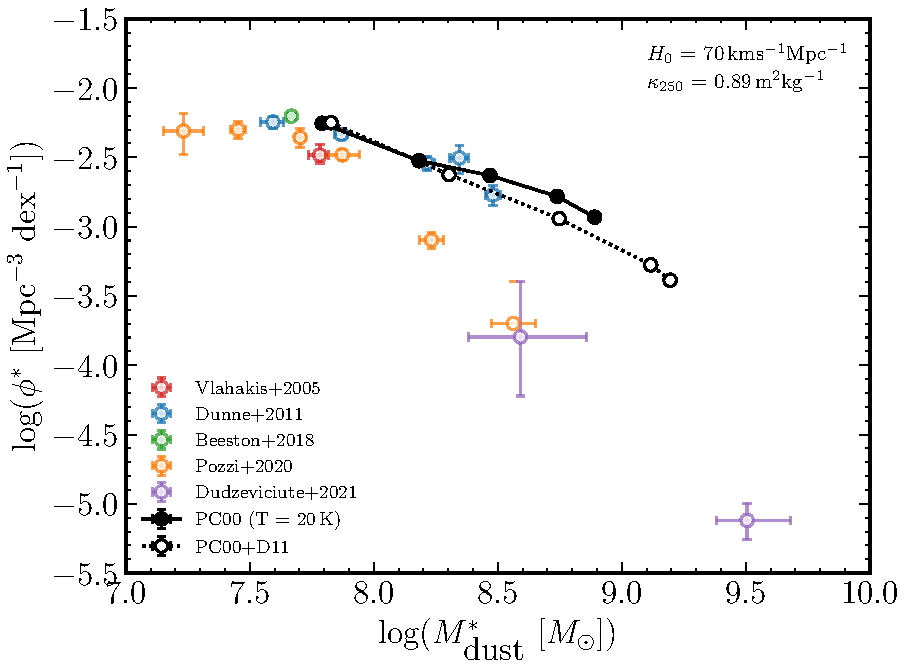
\includegraphics[width=0.8\columnwidth]{Figures/dmf_schechter_parameters.pdf}
	\caption[Distribution of $M_{\textrm{dust}}^*$ and $\phi^*$ from best fitting Schechter functions]{The distribution of $M_{\textrm{dust}}^*$ and $\phi^*$ for the two estimates of the DMF considered in this study ($T = 20\,$K shown as filled circles with solid lines and the \citealt{Dunne_2011} adaptation shown as open circles with dotted lines). The studies from the literature are the same as those given in Figure \ref{fig:dmf_schechter}. {\color{red}Add redshift indication.}}
	\label{fig:dmf_schechter_parameters}
\end{figure}

Figure \ref{fig:dmf_m_evolution} shows the variation in the characteristic dust mass as a function of redshift. We fit the observed relationships with a function of the form $\textrm{log}(M_{\textrm{dust}}^*) = \textrm{log}(M_{\textrm{dust,0}}^*)(1+z)^\gamma$. The best fitting functions are given by $\textrm{log}(M_{\textrm{dust}}^*) = (7.66\pm0.10)(1+z)^{0.30\pm0.03}$ when dust temperature is allowed to be free between $15$ and $25\,$K, and $\textrm{log}(M_{\textrm{dust}}^*) = (7.65\pm0.05)(1+z)^{0.24\pm0.01}$ when assuming $T_{\textrm{dust}} = 20\,$K. The $\textrm{log}(M_{\textrm{dust,0}})$ term represents a typical galaxy's dust mass at redshift zero, which is in excellent agreement between the two models. Using these fitted relationships we find that at $z = 1$, the galaxies detected by \textit{Herschel} were typically $60$ times dustier (or $\sim 25$ times when assuming $T_{\textrm{dust}} = 20\,$K) than today. \citealt{Dunne_2011} found that the most massive galaxies at the highest redshifts probed in their study, $z \sim 0.5$, have dust masses a factor of $5$ to $8$ larger than those at $z \sim 0$. At the same redshift, our empirical relationships find that the characteristic dust mass evolves by a factor of $6 - 10$, in good agreement with \citealt{Dunne_2011}.

\begin{figure}
	\centering
	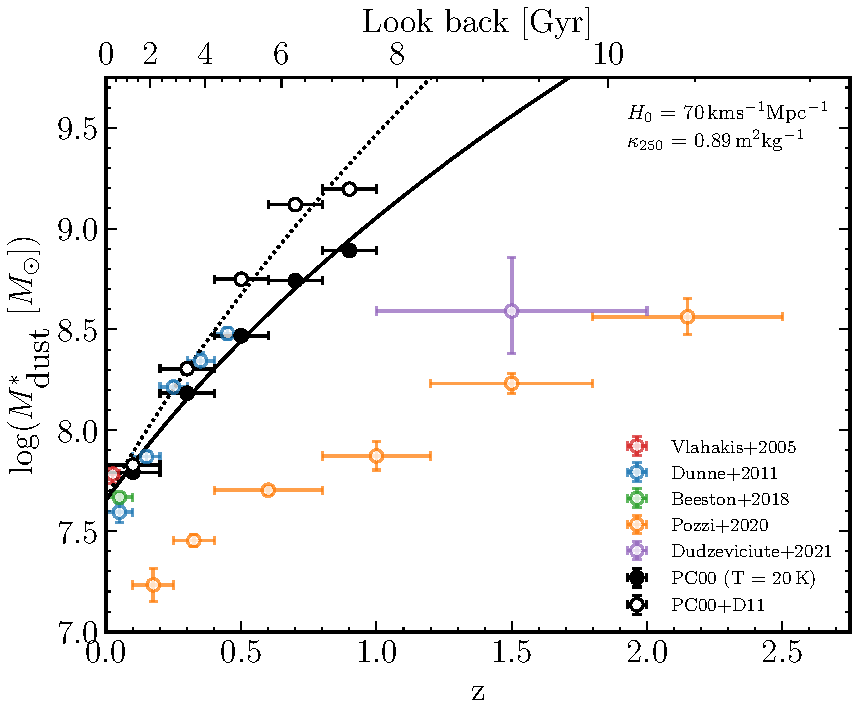
\includegraphics[width=0.7\columnwidth]{Figures/dmf_m_evolution.pdf}
	\caption[Evolution of the characteristic dust mass, $M_\textrm{dust}^*$, as a function of redshift]{The best fitting characteristic dust mass, $M_\textrm{dust}^*$, as a function of redshift. The coloured error bars have the same colour convention as Figure \ref{fig:dmf_schechter}. The solid and dotted lines represent best fitting relationships of the form $\textrm{log}(M_{\textrm{dust,0}}^*)(1+z)^\gamma$. For our $T_{\textrm{dust}} = 20\,$K DMF we find $\gamma = 0.24\pm0.01$ and $\gamma = 0.30\pm0.03$ when temperature is allowed to be free between $15\,$K and $25\,$K.}
	\label{fig:dmf_m_evolution}
\end{figure}

\subsection{Dust Mass Density}

Useful estimators of the dust content of galaxies across time are the integrated dust mass density (DMD), $\rho_{\textrm{dust}}$, and the dust mass density parameter, $\Omega_{\textrm{dust}}$. We integrate the DMFs in each redshift slice to calculate the total amount of dust in galaxies at different epochs. This integration is given by

\begin{equation}
    \rho_{\textrm{dust}} = \int_0^\infty M_{\textrm{dust}} \phi(M_{\textrm{dust}}) dM_{\textrm{dust}} = \Gamma(2+\alpha) M_{\textrm{dust}}^* \phi^*,
    \label{eq:dust_mass_density}
\end{equation}

\noindent where $\Gamma(x)$ represents the Gamma function, $\Gamma(x) = \int_0^\infty t^{x-1}e^{-t} dt$, and $\phi(M_{\textrm{dust}})$ has been substituted with the best fitting Schechter function. The dust mass density measured in this way is built upon a number of assumptions. First, it is assumed that the Schechter function is applicable at dust masses far below the range that has been directly measured. We could circumvent this problem by integrating to some common lower mass limit using the upper incomplete Gamma function, $\Gamma(x, z) = \int_z^\infty t^{x-1}e^{-t} dt$, however, all the studies considered here have varying levels of completeness at low masses and the integrated density without imposing this limit is negligibly different. As such, the DMD calculated using Equation \ref{eq:dust_mass_density} serves as a maximal estimate of the dust mass density. Second, the low mass slope is assumed to be constant with redshift such that the number density of lower mass galaxies does not change with time. This assumption has no motivation, but is not expected to have a significant impact on our dust mass densities as the majority of the contribution by mass comes from the much fewer, more massive galaxies. The dust mass density parameter is obtained from $\Omega_{\textrm{dust}} = \rho_{\textrm{dust}}/\rho_{\textrm{crit}}$ where $\rho_{\textrm{crit}} = 1.36\times10^{11}\,M_{\odot}$Mpc$^{-3}$ is the critical density for our assumed cosmology. The dust densities are listed in Table \ref{tab:schechter_parameters} and shown in Figure \ref{fig:dmd} alongside the measured values for the studies previously mentioned. 

\begin{figure}
	\centering
	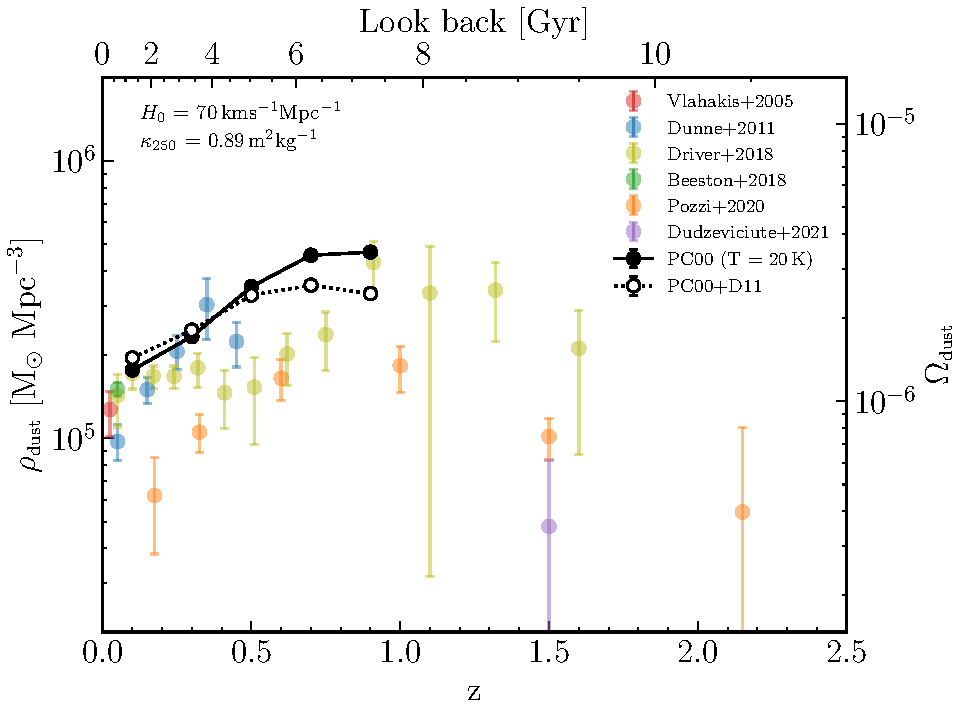
\includegraphics[width=0.8\columnwidth]{Figures/Figure_3_8.pdf}
	\caption[Integrated dust mass density as a function of redshift]{The integrated dust mass density and dust density parameter as a function of redshift for SGP galaxies, calculated using Equation \ref{eq:dust_mass_density}. The coloured error bars have the same colour convention as Figure \ref{fig:dmf_schechter}, with the addition of the study of \citealt{Driver_2018} (light green).}
	\label{fig:dmd}
\end{figure}

In reasonable agreement with \citealt{Dunne_2011}, we predict a rapid evolution in dust mass density in the local Universe, though it is notably less steep than the $(1+z)^{4.5}$ relationship observed in their study. Our measurement of the dust mass density suggests a factor $\sim 1.7 - 2.6$ increase between $0 < z < 0.2$ and $0.8 < z < 1$, beyond which the dust density remains roughly constant, suggesting a peak at redshifts around $0.8 - 1$. The rapid decrease in dust density from $z \sim 1$ to the present day may have a number of possible causes. First, the depletion of dust due to star formation, owing to the fact that evolution in dust mass and SFR are intrinsically related since stars form out of gas and the dust is expected to trace the interstellar gas reservoir. The decline may also be attributed to dust destruction or dust lost from the galaxy to the halo (\citealt{Dunne_2011}). In contrast to the prevailing \textit{Herschel} view, \citealt{Driver_2018} find a relatively flat density at redshifts $< 0.5$, though it is noted that the method used to calculate the incompleteness in their sample differs from the one used here, and by extension in \citealt{Dunne_2011}, which may be the root cause of the difference.

The prediction of a peak in the dust density varies among studies. \citealt{Driver_2018} study the stellar mass and dust mass density of GAMA sources out to redshift five, probing a large span of cosmic time and locating a peak in the dust density at $z \sim 1$. Despite an increase in the characteristic dust mass, \citealt{Dunne_2011} also observe a peak in their last redshift bin ($0.4 < z < 0.5$), however, this is based on a single dipped bin and has been linked to a systematic issue with photometric redshifts. Our two DMFs show signs that there is a peak in the dust density at a similar cosmic time to that of \citealt{Driver_2018}, but is also based on a single lower bin. In our study we only use photometric redshifts, but have factored the additional uncerainty this creates in our DMFs by running Monte Carlo simulations (Section \ref{sec:dmf_from_sgp}). We find that the contribution to the error budget from using photometric redshifts is of order the Poissonian errors and do not have a significant effect on the Schechter fitting and resulting dust mass densities. If, however, there were a systematic trend in the photometric redshifts, we might expect the observed evolution to change in steepness and/or shift the apparent peak to different redshifts.

\subsection{Comparison with the Star Formation Rate Density}

There is a direct link between star formation and the dust and gas content of galaxies. The Kennicutt-Schmidt relationship demonstrates the link between the gas and star formation rate surface densities of galaxies. Given that dust traces the gas in the ISM, there is a consequential link between dust content and the star formation activity. As a result, it is constructive to look at the dust mass density we observe from the galaxies in the SGP with the mean star formation rate in the Universe.

The redshift dependence of the cosmic star formation history given by \citealt{Madau_2014}, which takes the form of a double power law in $(1 + z)$, is based on the best fit to multiple UV and IR data sets representing the unobscured and obscured star formation densities. Combining these surveys provides a clear and comprehensive picture of the cosmic star formation activity. The best fitting function is given by

\begin{equation}
    \psi(z) = 0.015\frac{(1+z)^{2.7}}{1+[(1+z)/2.9]^{5.6}} [M_{\odot}\textrm{yr}^{-1}\textrm{Mpc}^{-3}].
    \label{eq:madau_sfrd}
\end{equation}

This expression implies a cosmic star formation history that scales as $(1 + z)^{-2.9}$ between $3 \lesssim z \lesssim 8$, a peak in the range $1.5 \lesssim z \lesssim 2$, and a decline of the form $(1 + z)^{2.7}$ to the present day. Figure \ref{fig:sfrd} shows our measurements of the dust mass density alongside the measurements of the mean star formation rate in the Universe. The offset between the two scales has been set to follow the relationship $\rho_{\textrm{dust}} = \rho_{\textrm{gas}}/\delta_{\textrm{gdr}} \sim \psi \times\tau_{\textrm{depl}}/\delta_{\textrm{gdr}}$, where we have assumed a typical depletion timescale, $\tau_{\textrm{depl}}$, of $1\,$Gyr (which is of a similar magnitude to individual galaxies on the star forming main sequence with $\textrm{log}(M_*) = 10.5$ at $z < 1$, as presented in \citealt{Tacconi_2020}) and a gas mass to dust mass ratio, $\delta_{\textrm{gdr}}$, of $100$. However, we do not intend for this to be interpreted as a suitable definition for the star formation density of SGP galaxies, rather as an approximation such that the two sets of measurements roughly coincide. 

\begin{figure}
	\centering
	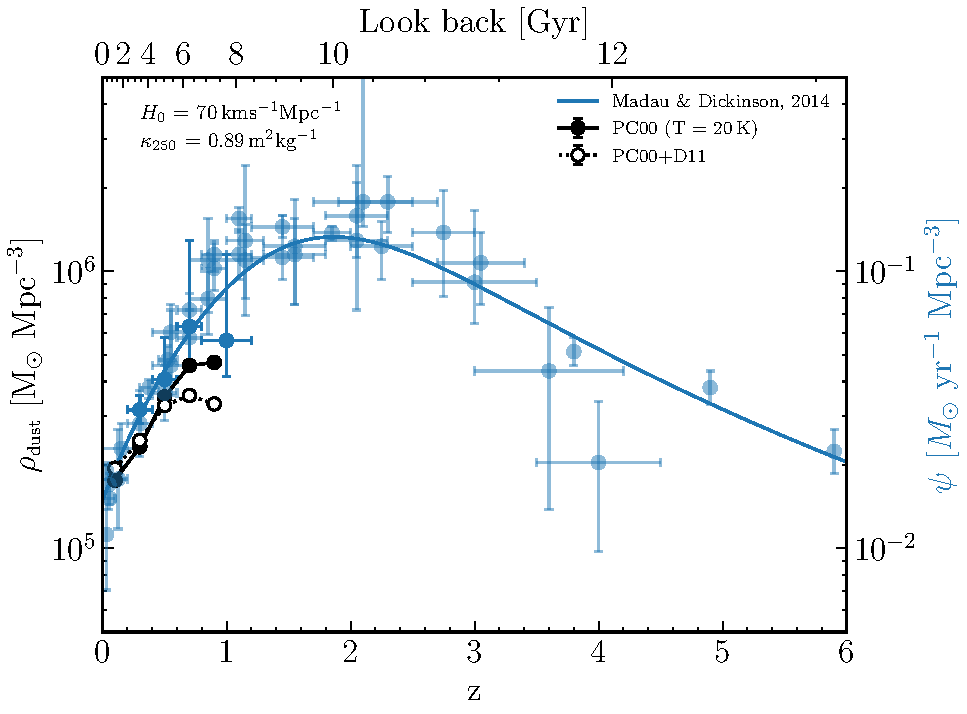
\includegraphics[width=0.74\columnwidth]{Figures/Figure_3_9.pdf}
	\caption[Comparison of dust mass density and the cosmic star formation rate density]{The integrated dust density of SGP galaxies as illustrated in Figure \ref{fig:dmd}. The blue error bars represent the various studies included in the fitting of \citealt{Madau_2014} for the cosmic star formation rate density (blue line). The two vertical axes have been scaled for illustrative purposes using $\rho_{\textrm{dust}} \sim \psi \times\tau_{\textrm{depl}}/\delta_{\textrm{gdr}}$, where we have assumed a typical depletion timescale of $500\,$Myr and a gas mass to dust mass ratio of $100$.}
    \label{fig:sfrd}
\end{figure}

The similarity in the evolutions of the dust mass density and the star formation rate density (SFRD) to the present day show that the two are intrinsically linked, and that the quantity of dust contained in galaxies is dependent on recent star formation. We know that dust can be formed in several ways, each with appreciably different timescales: the stellar winds of evolved asymptotic giant branch (AGB) and red giant branch (RGB) stars, which dominate dust production in high redshift galaxies for $150$ to $500\,$Myr after the onset of star formation (\citealt{Valiante_2009}); supernovae that dominate on timescales $< 1\,$Gyr (\citealt{Dwek_2007}); and continual grain growth in the ISM. Most processes involving dust can be linked directly to star formation, such as the formation of molecular clouds, stellar ejecta and supernovae, which all operate on timescales of order of the lifetime of massive stars (approximately less than $10\,$Myr, \citealt{Galliano_2018}). This means that it is not necessarily surprising that our dust mass density and the star formation rate density evolve in unison. Such short timescales would imply that the tentative peak in our evolution of $\rho_{\textrm{dust}}$ at $z \sim 1$, approximately $2 - 3\,$Gyr away from the peak in star formation density, is the result of some bias related to our use of photometric redshifts in estimating dust masses, but if true, would suggest a preference for dust production pathways that allow for a noticeable delay between the onset of star formation and dust production.

\section{Conclusions}

In this Chapter, we derived the dust masses of our SGP galaxies assuming an isothermal modified blackbody, setting limits on the temperature of the cold dust reservoir between $15$ and $25\,$K. From our sample we derived binned dust mass functions in redshift slices out to $z = 1$, representing approximately $8$ billion years in the past. We explored the differences between two measures of the DMF; one in which the cold dust is assumed to be constant at $20\,$K for all galaxies, and one where the dust temperature was allowed to vary within the predetermined bounds. The two methods yield similar results and are presented together without preference. From the evolution in the characteristic dust mass, we estimated that \textit{Herschel} detected galaxies were on average $25$ to $60$ times dustier at $z = 1$ than they are today. Next, we integrated both DMFs for the total amount of dust in \textit{Herschel} galaxies at various points in time. This dust mass density showed a rapid evolution from $z = 1$ to $z = 0$ of a factor approximately half, suggesting significant dust depletion due to star formation, dust destruction or dust lost to the halo over the past $8\,$Gyr. There is tentative evidence of a peak in the dust mass density at redshifts between $0.8$ and $1$, which if true, is shifted by $2 - 3\,$Gyr from the peak in the star formation rate density at $z \sim 2$. However, the most plausible cause of this downturn is our reliance on photometric redshifts that may have a systematic bias in this bin.

